% !TeX program = xelatex
% Compile twice from experiment-report/. Figures are in ../analysis/.
\documentclass[a4paper,12pt]{article}
\usepackage{fontspec,xeCJK}
\usepackage{graphicx,amsmath,amssymb,array,tabularx,booktabs}
\usepackage{float,caption,titlesec,geometry,xcolor,listings,xurl}
\usepackage[hidelinks]{hyperref}
\usepackage{bookmark}
\usepackage[section]{placeins}
\IfFontExistsTF{Songti SC}{\setCJKmainfont[AutoFakeBold=2.5]{Songti SC}}{\setCJKmainfont{FandolSong-Regular}}
\IfFontExistsTF{Heiti SC}{\setCJKsansfont[AutoFakeBold=2.5]{Heiti SC}}{\setCJKsansfont{FandolHei-Regular}}
\IfFontExistsTF{Kaiti SC}{\setCJKmonofont{Kaiti SC}}{\setCJKmonofont{FandolKai-Regular}}
\IfFontExistsTF{Times New Roman}{\setmainfont{Times New Roman}}{\setmainfont{TeX Gyre Termes}}
\IfFontExistsTF{Menlo}{\setmonofont{Menlo}[Scale=0.85]}{\setmonofont{Latin Modern Mono}[Scale=0.85]}
\XeTeXlinebreaklocale "zh"
\XeTeXlinebreakskip=0pt plus 1pt minus 0.1pt
\newcommand{\xiaoyi}{\fontsize{24pt}{36pt}\selectfont}
\newcommand{\erhao}{\fontsize{22pt}{28pt}\selectfont}
\newcommand{\xiaoer}{\fontsize{18pt}{24pt}\selectfont}
\newcommand{\xiaosan}{\fontsize{15pt}{22pt}\selectfont}
\newcommand{\sihao}{\fontsize{14pt}{21pt}\selectfont}
\newcommand{\xiaosi}{\fontsize{12pt}{18pt}\selectfont}
\geometry{left=3.18cm,right=3.18cm,top=2.54cm,bottom=2.54cm}
\titleformat{\section}{\sffamily\sihao\bfseries}{\thesection}{1em}{}
\titleformat{\subsection}{\sffamily\xiaosi\bfseries}{\thesubsection}{1em}{}
\titlespacing*{\section}{0pt}{0.9em}{0.45em}
\titlespacing*{\subsection}{0pt}{0.7em}{0.3em}
\setlength{\parindent}{2em}
\setlength{\parskip}{0.25em}
\setlength{\emergencystretch}{2em}
\renewcommand{\arraystretch}{1.18}
\captionsetup{font=small,labelfont=bf,labelsep=colon}
\renewcommand{\figurename}{Figure}
\renewcommand{\tablename}{Table}
\newcolumntype{Y}{>{\raggedright\arraybackslash}X}
\definecolor{codebg}{RGB}{30,30,30}
\definecolor{codefg}{RGB}{214,220,229}
\lstset{backgroundcolor=\color{codebg},basicstyle=\color{codefg}\ttfamily\footnotesize,
 breaklines=true,columns=fullflexible,keepspaces=true,frame=single,
 rulecolor=\color{codebg},showstringspaces=false,aboveskip=0.7em,belowskip=0.7em}
\urlstyle{tt}
\hypersetup{pdftitle={山梨酸紫外光谱与核磁共振谱的计算},pdfauthor={叶青杨}}
\newcommand{\ReportTitle}{山梨酸紫外光谱与核磁共振谱的计算}

\begin{document}
\begin{titlepage}
\centering
\IfFileExists{image/zju.png}{\includegraphics[width=3.18cm]{image/zju.png}\par}{}
\vspace{0.8cm}
{\xiaoyi\bfseries 浙江大学量子化学实验\par}
\vspace{1cm}
{\sffamily\xiaoer \ReportTitle\par}
\vspace{0.7cm}
{\sffamily\erhao\bfseries 实\\[0.32cm]验\\[0.32cm]报\\[0.32cm]告\par}
\vfill
{\sihao 参加学生：叶青杨\par}
\vspace{1cm}
{\xiaoer\bfseries 浙江大学化学实验教学中心\par}
\vspace{0.5cm}
{\xiaoer\bfseries 2026年10月8日\par}
\end{titlepage}
\setcounter{page}{1}
\begin{center}
{\sffamily\xiaosan\bfseries \ReportTitle\par}
\vspace{0.4em}
{\xiaosi 叶青杨\par}
\end{center}
\xiaosi

\section{实验目的}
以 $(2E,4E)$-己二烯酸（山梨酸，$\mathrm{C_6H_8O_2}$）为对象，比较不同构象的稳定性，学习含时密度泛函理论（TD-DFT）和规范无关原子轨道（GIAO）方法，计算紫外吸收、核磁屏蔽及自旋耦合常数，分析构象变化及羧酸双氢键缔合对光谱的影响\cite{course}。

\section{实验原理}
\subsection{几何优化与构象比较}
在相同方法与基组下，几何优化给出势能面上的驻点。含 $N$ 个原子的非线性分子有 $3N-6$ 个内部振动模式；山梨酸单体和二聚体分别有 42 和 90 个正常模式，全部频率为正表明它们是局部极小点。同一组成的候选构象间，电子能差定义为
\begin{equation}
\Delta E_i=(E_i-E_{\min})\times2625.49964\ \mathrm{kJ\,mol^{-1}},
\end{equation}
其中 $E$ 以 Hartree 为单位，$E_{\min}$ 为所比较构象中的最低电子能。

\subsection{垂直电子跃迁与紫外吸收}
在基态平衡几何 $R_0$ 上，垂直吸收能为
\begin{equation}
\Delta E_n^{\mathrm{abs}}=E_n(R_0)-E_0(R_0),\qquad
\lambda_n=\frac{hc}{\Delta E_n}.
\end{equation}
TD-DFT 给出激发能和振子强度 $f_n$，分别对应吸收位置和跃迁强弱。SMD 将溶剂表示为连续介质，用于描述溶剂对电子结构及激发能的影响。

\subsection{核磁屏蔽与自旋耦合}
各向同性磁屏蔽常数为屏蔽张量迹的三分之一：
\begin{equation}
\sigma_{\mathrm{iso}}=\tfrac13(\sigma_{xx}+\sigma_{yy}+\sigma_{zz}).
\end{equation}
相对于参照物的化学位移近似为 $\delta_i\simeq\sigma_{\mathrm{ref}}-\sigma_i$。理论体系之间比较屏蔽值 $\sigma$（ppm）；与实验比较时，以同种核的甲基信号为参照，通过位移差消去参照物的屏蔽常数：
\begin{equation}
\Delta\delta_i^{\mathrm{exp}}=\delta_i^{\mathrm{exp}}-\delta_{\mathrm{CH_3}}^{\mathrm{exp}},\qquad
\Delta\delta_i^{\mathrm{calc}}=\overline{\sigma}_{\mathrm{CH_3}}^{\mathrm{calc}}-\sigma_i^{\mathrm{calc}}.
\label{eq:relative-shift}
\end{equation}
核间自旋耦合以 $J$（Hz）表示，其大小与成键关系和分子几何有关。

\clearpage
\section{计算方法与实验步骤}
\subsection{构象建立}
保持两个双键的 E 构型，改变羧基相对共轭链的朝向和 O--H 取向，建立三个初始构象，分别记为 conf-01、conf-02 和 conf-03。计算采用 Gaussian 16 A.03，分子电荷为 0，自旋多重度为 1。

由 conf-01 与 conf-02 组合建立 01/01、01/02 和 02/02 三种环状双氢键二聚体。二聚体组成为 $\mathrm{C_{12}H_{16}O_4}$，含 32 个原子、120 个电子，均为中性单重态；两个单体片段分别采用 1--16 和 17--32 的原子编号。

\subsection{基态优化与频率分析}
三个构象采用同一 PBE0/6-31G(d) 水平进行气相无约束优化和频率分析。Gaussian 中 PBE0 对应 \texttt{PBE1PBE}，\texttt{6-31G(d)} 与课程采用的 \texttt{6-31G*} 等价。主要输入如下：
\begin{lstlisting}
#p PBE1PBE/6-31G(d) Opt=(Tight,CalcFC) Freq
   SCF=(Tight,XQC) Int=UltraFine NoSymm
\end{lstlisting}
根据优化结构比较键长和二面角，并通过频率分析判断局部稳定性。热化学量采用 298.15 K、1 atm 下的气相刚性转子--谐振子（RRHO）近似，未作低频修正。

二聚体采用相同的气相优化与频率计算方法，比较其成键关系、质子位置、双氢键几何及极小值是否重复，再进行性质计算。

\subsection{紫外与核磁计算}
以能量最低的 conf-02 为基准，同时计算能量接近的 conf-01。固定各自的气相优化几何，采用 SMD 乙醚模型计算最低的 20 个激发单重态：
\begin{lstlisting}
#p PBE1PBE/6-31G(d) TD=(Singlets,NStates=20)
   SCRF=(SMD,Solvent=DiethylEther)
   SCF=(Tight,XQC) Int=UltraFine NoSymm
\end{lstlisting}
核磁屏蔽和自旋耦合常数在气相中计算：
\begin{lstlisting}
#p PBE1PBE/6-31G(d) NMR=(GIAO,SpinSpin,Mixed)
   SCF=(Tight,XQC) Int=UltraFine NoSymm
\end{lstlisting}
\texttt{Mixed} 方法以解收缩并加入紧函数的基组计算 Fermi 接触项，其余耦合贡献使用原基组，以改善近核电子密度对耦合常数的描述\cite{nmr,deng}。

三个稳定二聚体沿用相同的泛函、基组及溶剂设置，UV 计算最低 40 个激发单重态，NMR 采用同一气相 \texttt{GIAO/SpinSpin/Mixed} 方法。UV 曲线在共同覆盖的 $160$--$350\ \mathrm{nm}$ 区间比较，各结构分别作图。

实验比较使用公开文献中的山梨酸 UV、$^1$H 和 $^{13}$C 数据。NMR 相对位移按式\eqref{eq:relative-shift}计算：甲基氢取三个静态屏蔽值的平均值，近似描述快速转动；二聚体以两个甲基中同种核的平均屏蔽为共同参照，保留两个片段的各核位置。烯氢或烯碳的平均绝对偏差定义为 $\mathrm{MAE}=M^{-1}\sum_{i=1}^{M}|\Delta\delta_i^{\mathrm{calc}}-\Delta\delta_i^{\mathrm{exp}}|$，单体 $M=4$、二聚体 $M=8$；羟基氢和羧基碳另行比较。

\subsection{数据与程序}
本实验的计算输入、结果数据、实验参考数据的来源记录及后处理脚本整理于项目仓库：
\begin{center}
\url{https://github.com/populuscathayana/Quantum2}
\end{center}
按照仓库中的 \texttt{README.md} 和 \texttt{ENVIRONMENT.md}，可从已有计算结果重新生成光谱、比较表格和轨道图，无需重复量子化学计算。原创代码与文档采用 MIT 许可；引用的实验参考数据遵循原始来源的使用与引用条件。

\clearpage
\section{结果与分析}
\subsection{优化结构及相对稳定性}
三个构象均有 42 个正频率，无虚频，表明它们是所用计算水平下的局部极小点。优化后两个双键均保持 E 构型，共轭重原子骨架近乎共面。
\begin{figure}[H]
\centering
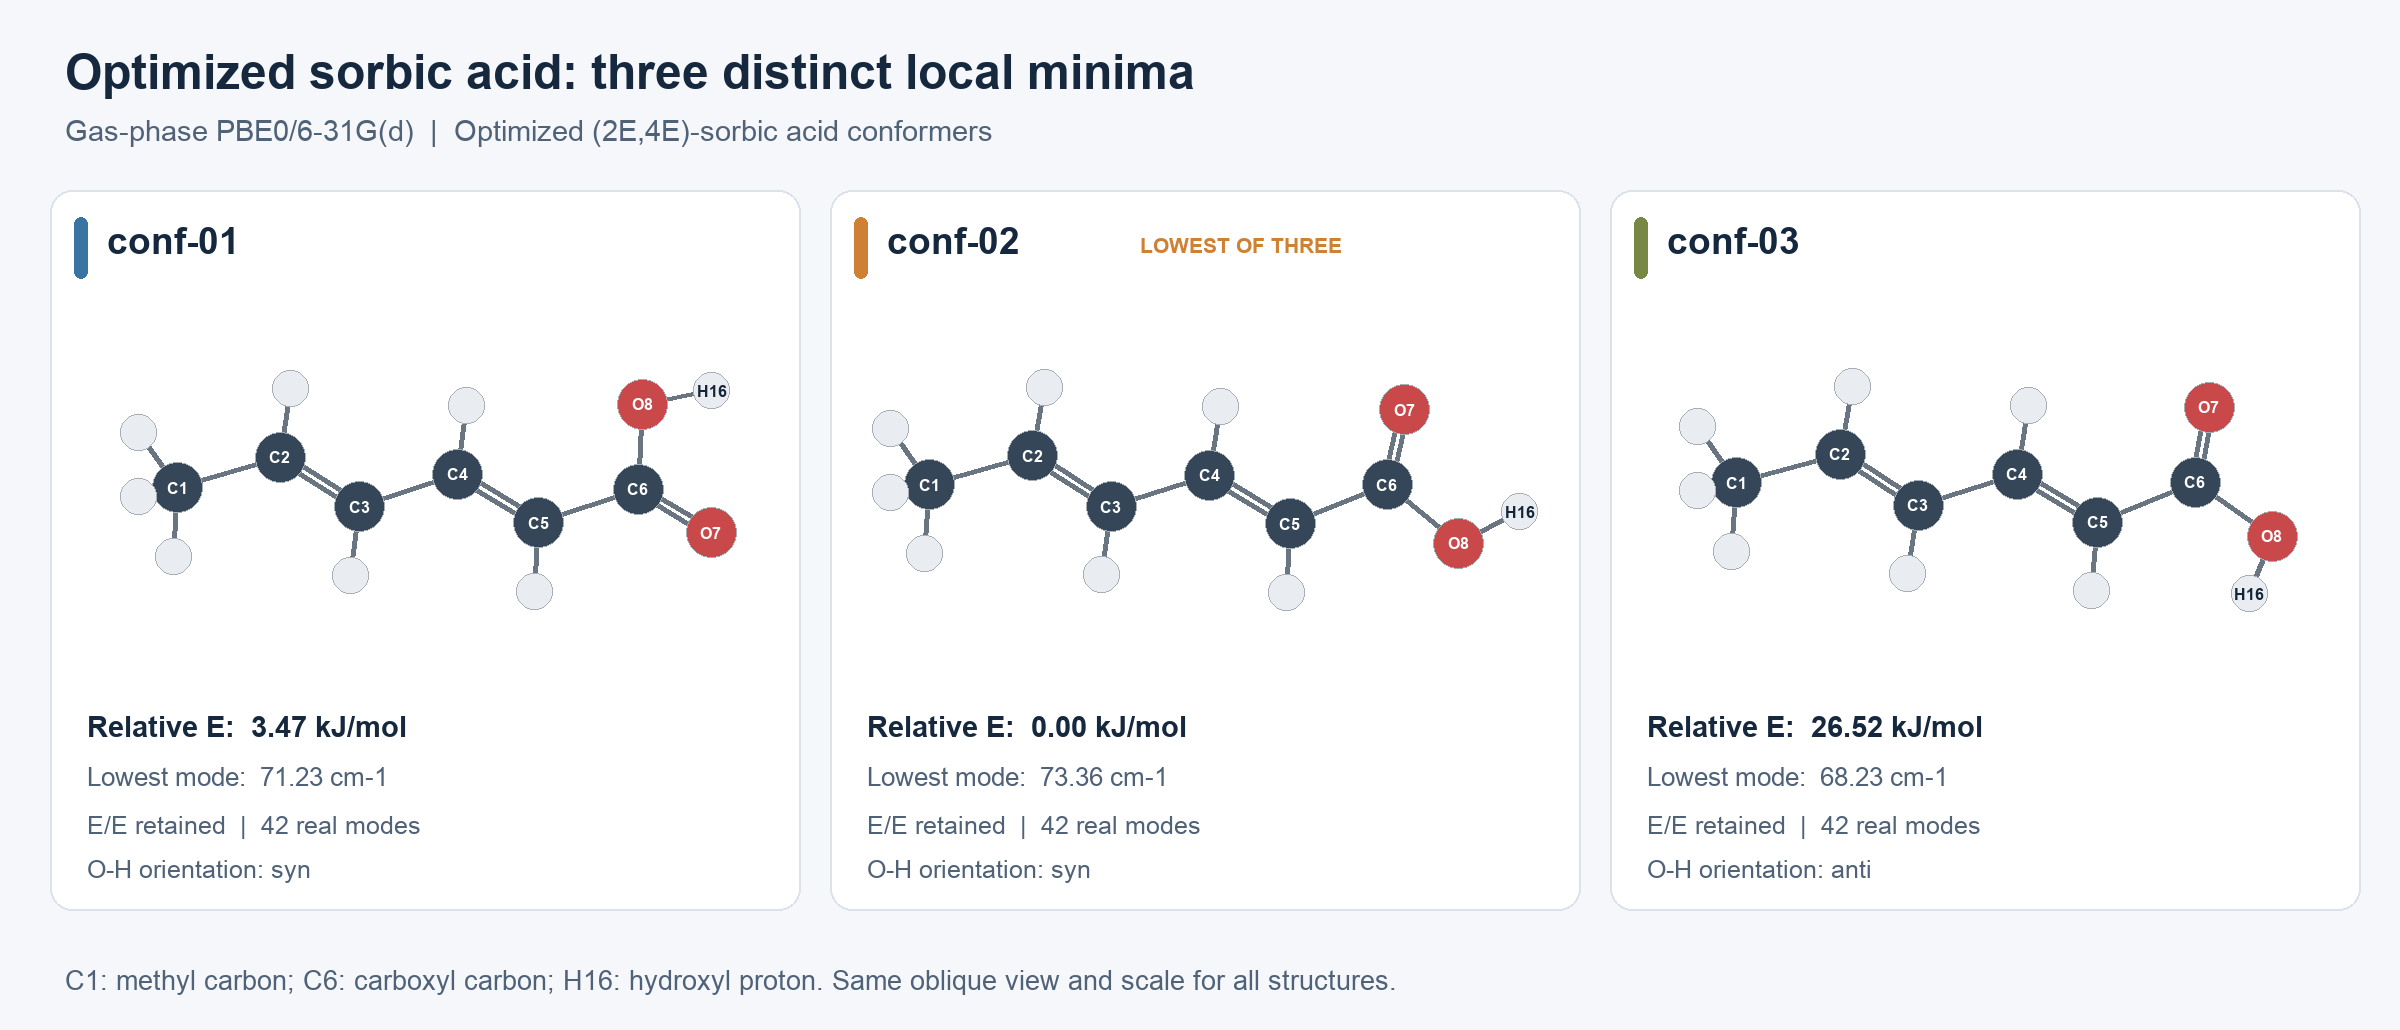
\includegraphics[width=\linewidth]{../analysis/stage1/optimized-structures.png}
\caption{山梨酸的三个优化构象。C1 为甲基碳，C6 为羧基碳，O7、O8 分别为羰基氧和羟基氧，H16 为羟基氢。}
\label{fig:structures}
\end{figure}
\begin{table}[H]
\centering\small
\caption{气相 PBE0/6-31G(d) 构象能量与最低振动频率。}
\begin{tabular}{lrrrr}
\toprule
构象 & $E/\mathrm{Hartree}$ & $\Delta E$ & $\Delta G$ & $\nu_{\min}$\\
 & & \multicolumn{2}{c}{$\mathrm{kJ\,mol^{-1}}$} & $\mathrm{cm^{-1}}$\\
\midrule
conf-01 & $-383.444694443$ & 3.4675 & 3.1270 & 71.2331\\
conf-02 & $-383.446015158$ & 0.0000 & 0.0000 & 73.3640\\
conf-03 & $-383.435914364$ & 26.5196 & 24.8819 & 68.2331\\
\bottomrule
\end{tabular}
\end{table}
conf-01 与 conf-02 的 C4--C5--C6--O7 二面角分别约为 $180^\circ$ 与 $0^\circ$，两者的羧基朝向不同；conf-02 与 conf-03 的 O7--C6--O8--H16 二面角分别约为 $0^\circ$ 与 $180^\circ$，主要区别在于 O--H 取向。

conf-02 的 C2=C3、C4=C5 键长分别为 1.3435、1.3453 \AA，连接两者的 C3--C4 为 1.4430 \AA，共轭链中仍可见长短键交替。羧基 C6=O7 为 1.2136 \AA，C6--O8 为 1.3514 \AA。

电子能和气相自由能均以 conf-02 最低。conf-01 与其电子能仅相差 $3.47\ \mathrm{kJ\,mol^{-1}}$，因此将二者纳入光谱比较；conf-03 在所比较的三个构象中能量明显较高。

\clearpage
\subsection{环状二聚体的结构与稳定性}
三种二聚体均保留两个山梨酸片段的 E/E 构型及两条 O--H$\cdots$O 氢键，未发生质子转移或异常成键。每种结构的 90 个振动频率均为正，分别对应不同的局部极小值。
\begin{figure}[H]
\centering
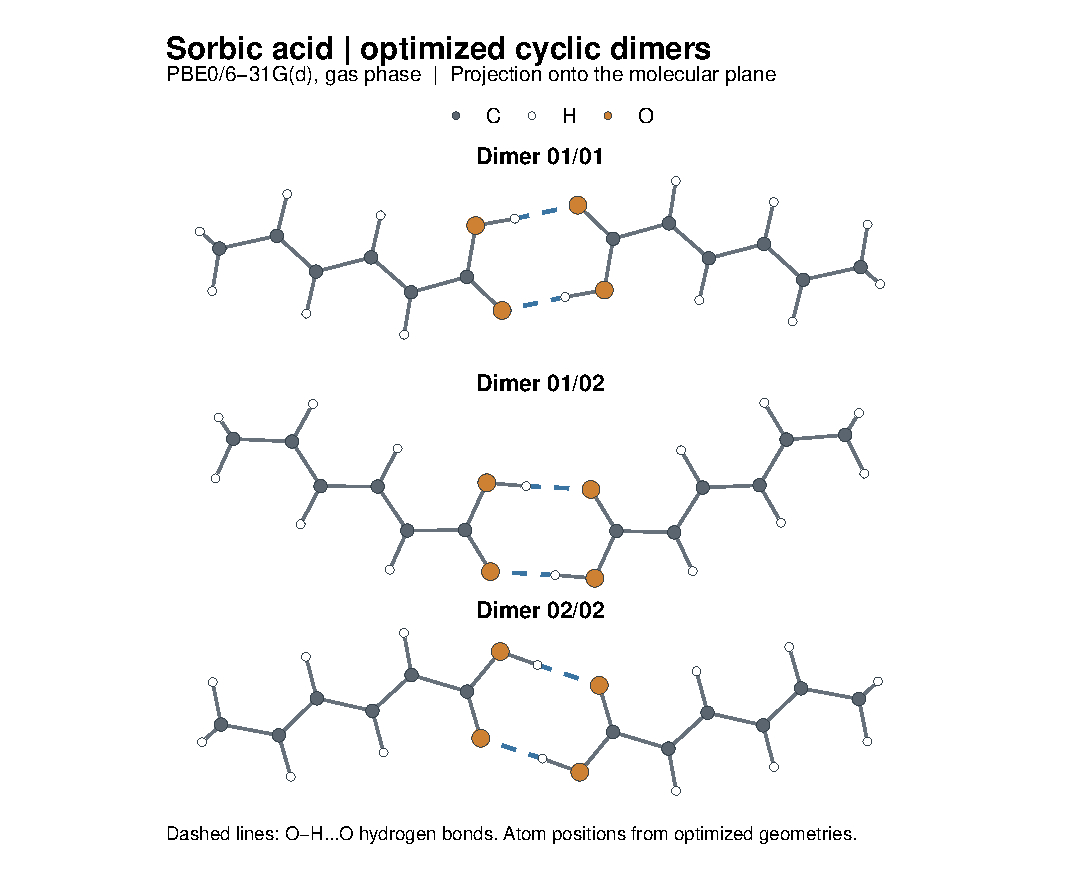
\includegraphics[width=\linewidth]{../analysis/comparison/dimer-structures.pdf}
\caption{三种环状二聚体的优化结构在重原子最佳拟合平面上的投影，虚线表示氢键。}
\label{fig:dimers}
\end{figure}
\begin{table}[H]
\centering\small
\caption{二聚体的电子能、相对能量和最低振动频率。相对能量以 02/02 为零点。}
\begin{tabular}{lrrr}
\toprule
二聚体 & $E/\mathrm{Hartree}$ & $\Delta E/\mathrm{kJ\,mol^{-1}}$ & $\nu_{\min}/\mathrm{cm^{-1}}$\\
\midrule
01/01 & $-766.923589459$ & 4.0718 & 11.6576\\
01/02 & $-766.924328476$ & 2.1315 & 21.3731\\
02/02 & $-766.925140336$ & 0.0000 & 13.8442\\
\bottomrule
\end{tabular}
\end{table}
两条氢键的 O$\cdots$O 距离为 2.6411--2.6515 \AA，H$\cdots$O 距离为 1.6358--1.6476 \AA。三个候选中 02/02 的电子能最低。最低振动频率仅为 $12$--$21\ \mathrm{cm^{-1}}$，反映了较柔软的分子间运动，因此这里主要比较电子能和氢键几何。

\clearpage
\subsection{紫外吸收光谱}
conf-02 的最强跃迁为 $S_0\rightarrow S_2$，激发能 $4.8160\ \mathrm{eV}$，波长 $257.44\ \mathrm{nm}$，振子强度 $f=0.9375$。其最低激发单重态 $S_1$ 位于 $262.36\ \mathrm{nm}$，但 $f=0.0001$，故最低能跃迁并不对应最强吸收。conf-01 的最强跃迁同为 $S_2$，位于 $256.20\ \mathrm{nm}$，两种单体的主吸收带较接近。
\begin{figure}[H]
\centering
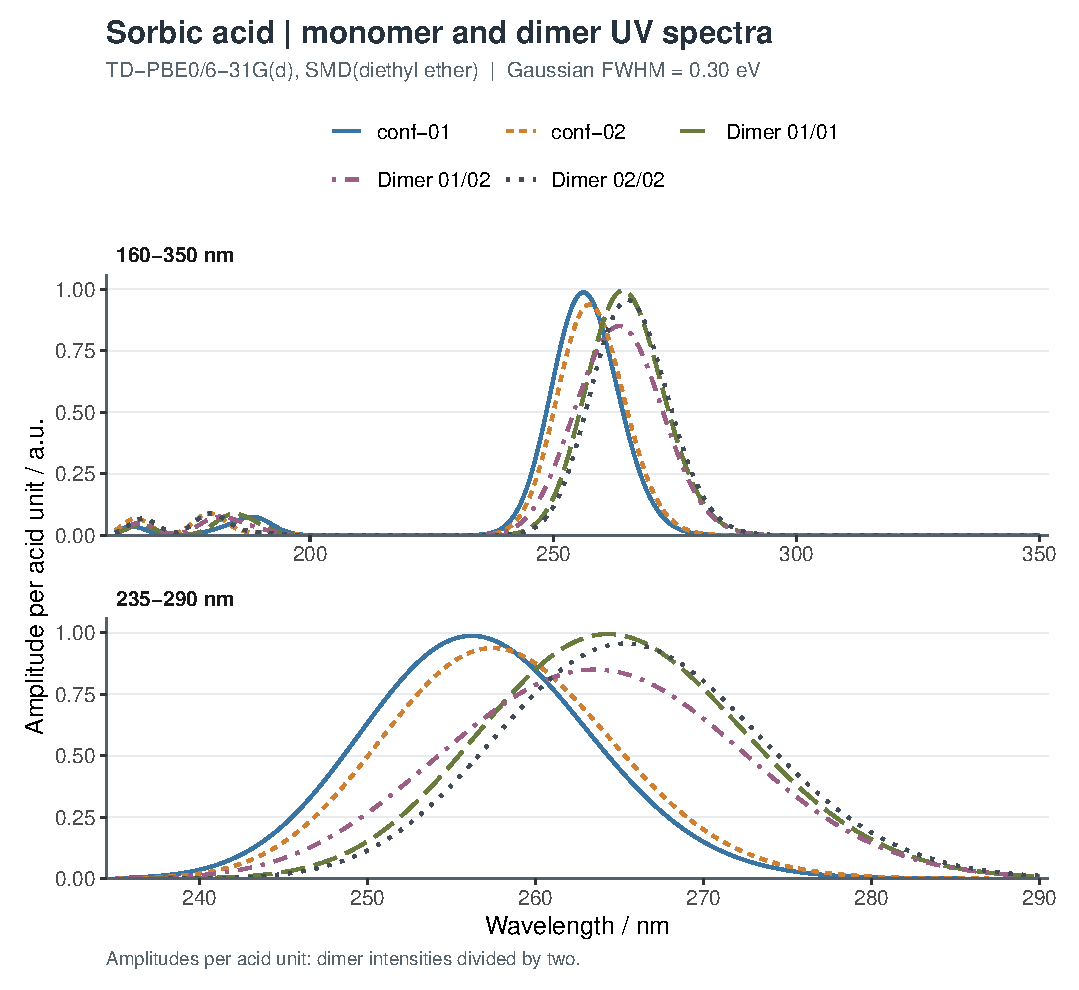
\includegraphics[width=\linewidth]{../analysis/comparison/uv-comparison.pdf}
\caption{两种单体及三种二聚体的 UV 比较。下图放大主吸收区；二聚体强度除以 2，以每个山梨酸单元为比较基准，各曲线未分别归一化。}
\label{fig:uv}
\end{figure}
绘图采用
\begin{equation}
I(E)=\frac{1}{n_{\mathrm{acid}}}\sum_{n=1}^{N_{\mathrm{state}}}f_n\exp\!\left[-4\ln2\frac{(E-E_n)^2}{w_E^2}\right],
\quad w_E=0.30\ \mathrm{eV},\quad E=hc/\lambda.
\end{equation}
其中单体的 $n_{\mathrm{acid}}=1$、$N_{\mathrm{state}}=20$，二聚体分别为 2 和 40。展宽在能量坐标下进行，再按 $E=hc/\lambda$ 映射到波长坐标，纵轴为任意单位的吸收振幅。所选谱区的最高能量比所有体系的已计算态上限至少低 $0.90\ \mathrm{eV}$，以减少态数截断对展宽曲线边缘的影响。

\begin{table}[H]
\centering\small
\caption{最强离散跃迁与展宽后主峰的比较。$f$ 为每个完整单体或二聚体的振子强度。}
\begin{tabular}{lrrrr}
\toprule
体系 & 激发态 & $\lambda/\mathrm{nm}$ & $f$ & 展宽峰位 / nm\\
\midrule
conf-01 & 2 & 256.20 & 0.9872 & 256.20\\
conf-02 & 2 & 257.44 & 0.9375 & 257.44\\
01/01 & 1 & 266.91 & 1.1871 & 264.32\\
01/02 & 1 & 267.41 & 0.9683 & 263.53\\
02/02 & 1 & 267.38 & 1.3038 & 265.31\\
\bottomrule
\end{tabular}
\end{table}
二聚体主吸收带均向长波方向移动。01/01 相对 conf-01 的展宽峰红移 $8.12\ \mathrm{nm}$，02/02 相对 conf-02 红移 $7.87\ \mathrm{nm}$，大于两种单体间 $1.24\ \mathrm{nm}$ 的差别。二聚体中多个相邻跃迁共同构成主吸收带，使展宽后的峰位与最强离散跃迁有所差异。

\clearpage
\subsection{与实验 UV 参考谱的比较}
采用 NIST Chemistry WebBook 收录的山梨酸 UV 数据\cite{nistuv}，原始来源为 Timmons 的 \textit{UV Atlas of Organic Compounds}（1966），谱图编号为 RAS UV No. 19947。数据包含 $200.07$--$292.23\ \mathrm{nm}$ 的 126 个点，纵坐标为 $\log_{10}\varepsilon$，故先取 $\varepsilon=10^{\log_{10}\varepsilon}$，再将实验和各理论曲线分别除以自身最大值。理论曲线保持原始波长和 $0.30\ \mathrm{eV}$ 展宽。该条目未注明溶剂、浓度和温度，以下比较峰位和归一化包络。
\begin{figure}[H]
\centering
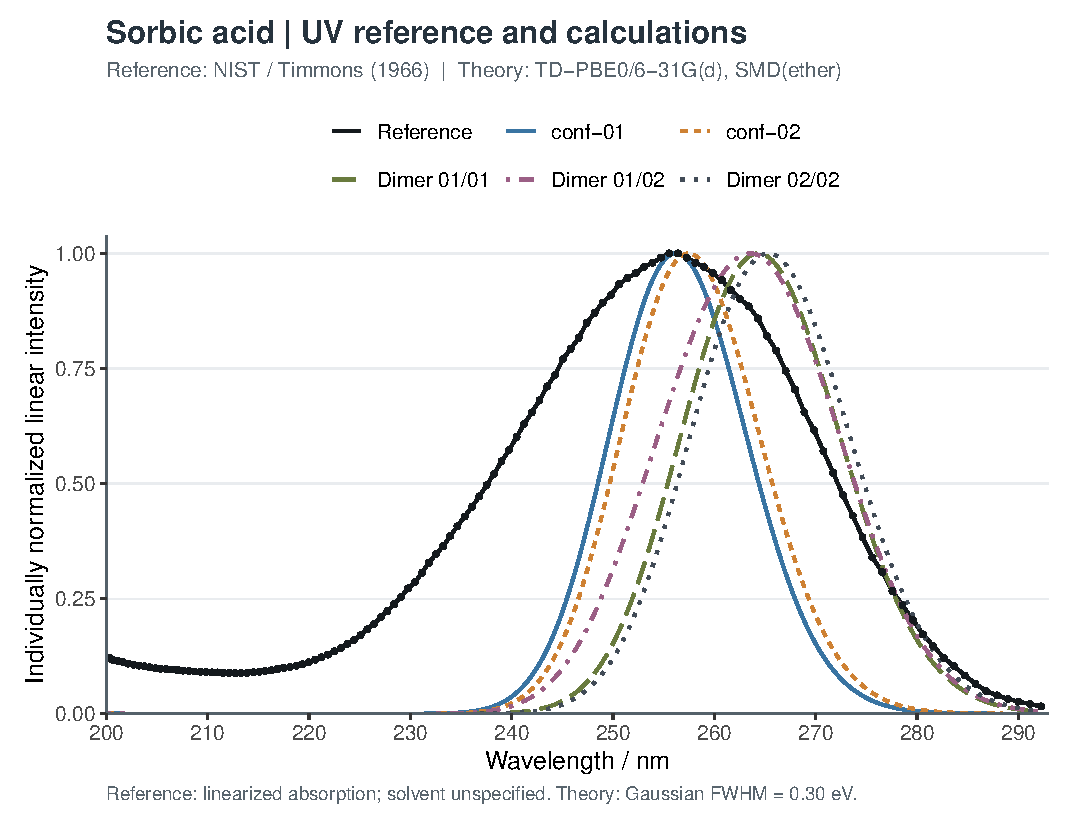
\includegraphics[width=\linewidth]{../analysis/experimental/uv-experiment-comparison.pdf}
\caption{实验 UV 参考数据与理论曲线。黑点为 NIST 数据，连线连接相邻数据点；各曲线的线性强度分别归一化。}
\label{fig:uvexp}
\end{figure}
参考谱在 $255.56$ 和 $256.41\ \mathrm{nm}$ 两点均达到最大值，峰位约为 $256.0\ \mathrm{nm}$。conf-01 与 conf-02 的峰位分别为 256.20 和 $257.44\ \mathrm{nm}$，均接近该吸收区；三个二聚体则位于 $263.53$--$265.31\ \mathrm{nm}$，比参考峰偏长波约 $7.5$--$9.3\ \mathrm{nm}$。就主吸收峰位而言，两种单体模型与参考谱更为接近。

对线性强度的半峰高交点作线性插值，参考带的半高全宽约为 $34.6\ \mathrm{nm}$，两个单体则分别为 $15.9$ 和 $16.1\ \mathrm{nm}$。理论曲线明显偏窄，说明除垂直跃迁位置外，振动包络和溶液环境分布也是描述实验带形的重要因素。

\clearpage
\subsection{主要跃迁的轨道归属}
$S_2$ 的主要组态为 $30\rightarrow31$，跃迁振幅为 0.70480；$S_1$ 主要包含 $29\rightarrow31$（0.69158）及 $29\rightarrow32$（$-0.13452$）。相关轨道如图\ref{fig:mo}所示。
\begin{figure}[H]
\centering
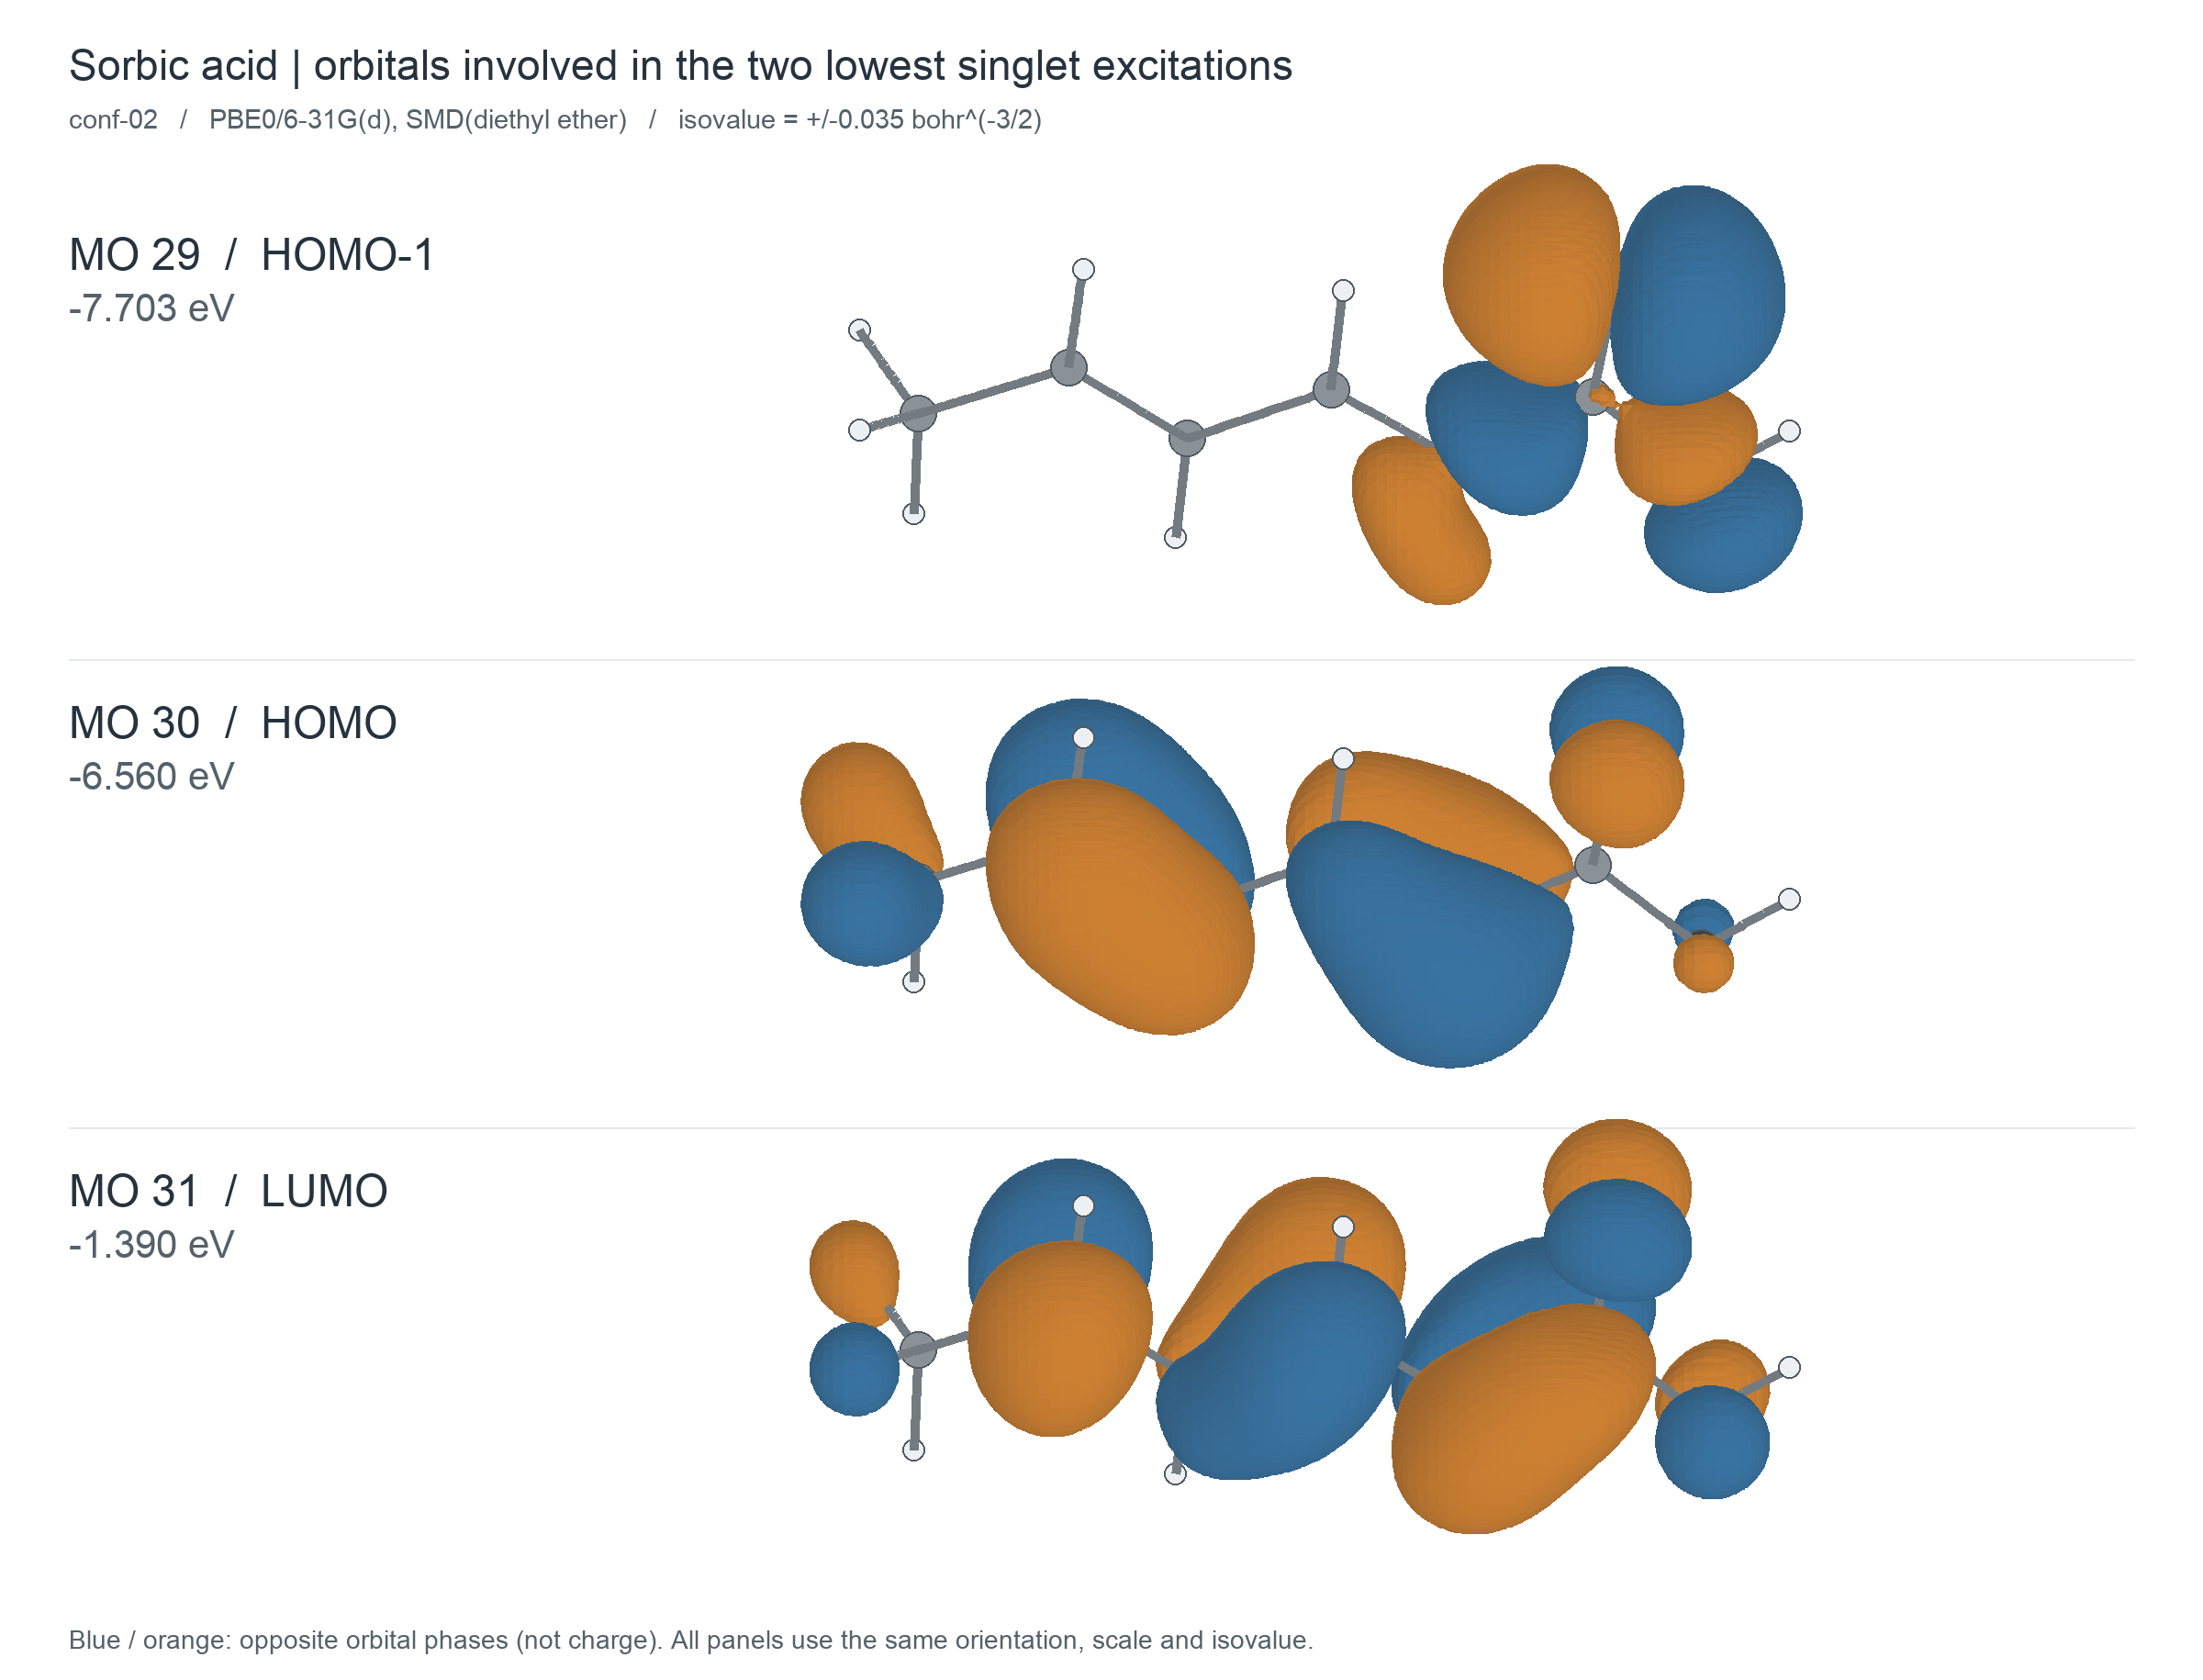
\includegraphics[width=\linewidth]{../analysis/stage2/frontier-orbitals.png}
\caption{MO 29、HOMO（MO 30）与 LUMO（MO 31）。等值面为 $\pm0.035\ \mathrm{bohr^{-3/2}}$，蓝色与橙色表示轨道的相反相位。}
\label{fig:mo}
\end{figure}
HOMO 和 LUMO 均沿同一共轭骨架分布，关于重原子平面近似反对称，呈现 $\pi$ 型轨道特征；LUMO 的相位交替体现反键性质。因此 $S_2$ 主要归属为共轭体系内部的 $\pi\rightarrow\pi^*$ 跃迁，轨道图中未见明显的空间分离电荷转移特征。MO 29 的分布更集中于含氧端，具有非键轨道特征，$S_1$ 可定性归属为以 $n\rightarrow\pi^*$ 为主的弱跃迁。

溶剂化基态 HOMO 与 LUMO 的轨道能分别为 $-6.560$ 和 $-1.390\ \mathrm{eV}$，能隙约 $5.170\ \mathrm{eV}$，大于 TD-DFT 给出的 $4.816\ \mathrm{eV}$ 激发能。这是因为 TD-DFT 激发能包含电子响应和组态耦合，并非简单的单电子轨道能量差。

\clearpage
\subsection{核磁屏蔽谱与原子指认}
图\ref{fig:nmr}分别显示氢核与碳核的屏蔽谱。H9--H11 为 C1 上的甲基氢，H12--H15 依次连接 C2--C5，H16 为羟基氢。
\begin{figure}[H]
\centering
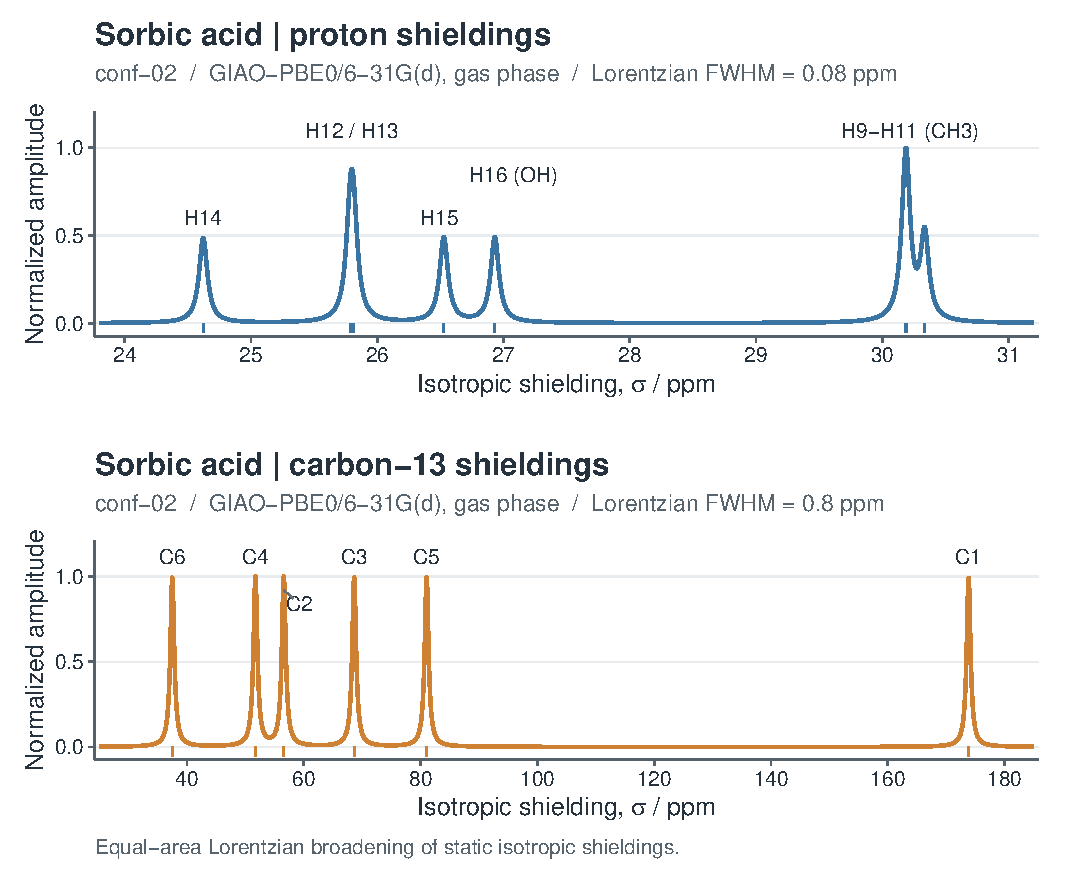
\includegraphics[width=\linewidth]{../analysis/stage2/nmr-shielding-spectra.pdf}
\caption{conf-02 的 $^1$H 与 $^{13}$C 屏蔽谱。短棒标出各核的屏蔽值，曲线分别归一化，未加入 $J$ 耦合裂分。}
\label{fig:nmr}
\end{figure}
每个核以等面积 Lorentz 线型展宽：
\begin{equation}
L(\sigma)=\sum_i\frac{w_\sigma/(2\pi)}{(\sigma-\sigma_i)^2+(w_\sigma/2)^2},
\end{equation}
其中氢谱与碳谱的半高全宽分别取 0.08 与 0.80 ppm。各核使用相同的积分面积，峰的重叠反映屏蔽值的接近程度。

\clearpage
\begin{table}[H]
\centering\small
\caption{conf-02 各原子的各向同性屏蔽常数。}
\begin{tabular}{llrllr}
\toprule
原子 & 环境 & $\sigma/\mathrm{ppm}$ & 原子 & 环境 & $\sigma/\mathrm{ppm}$\\
\midrule
C1 & 甲基碳 & 173.8328 & H9 & C1--H & 30.1873\\
C2 & 烯碳 & 56.5682 & H10 & C1--H & 30.1873\\
C3 & 烯碳 & 68.6187 & H11 & C1--H & 30.3356\\
C4 & 烯碳 & 51.7120 & H12 & C2--H & 25.7862\\
C5 & 烯碳 & 81.0282 & H13 & C3--H & 25.8118\\
C6 & 羧基碳 & 37.4764 & H14 & C4--H & 24.6220\\
O7 & 羰基氧 & $-23.8327$ & H15 & C5--H & 26.5273\\
O8 & 羟基氧 & 141.7341 & H16 & O8--H & 26.9311\\
\bottomrule
\end{tabular}
\end{table}
碳核中，甲基碳 C1 的屏蔽最强，羧基碳 C6 最弱，对应于 C1 位于高场、C6 位于低场。四个烯碳因相对羧基和甲基的位置不同而具有不同屏蔽。氢核中，甲基氢为 $30.19$--$30.34\ \mathrm{ppm}$，烯氢为 $24.62$--$26.53\ \mathrm{ppm}$，H14 屏蔽最弱。H12 与 H13 的屏蔽值很接近，因此在所选展宽下明显重叠。

静态构象中 H9/H10 与 H11 的屏蔽不完全相同，而溶液中的快速甲基转动会使其趋于平均。羟基氢的屏蔽值为 $26.9311\ \mathrm{ppm}$，溶液中的氢键和质子交换还会影响其屏蔽与谱线形状。

\subsection{自旋耦合与双键构型}
\begin{table}[H]
\centering\small
\caption{conf-02 的总 $J$ 耦合常数及文献实验值（Hz）。实验数据来自 $\mathrm{CDCl_3}$ 溶液\cite{nishiyama}；横线表示原表未给出该原子对的独立耦合值。}
\label{tab:couplings}
\begin{tabularx}{\linewidth}{lrrY}
\toprule
原子对 & 计算值 & 实验值 & 结构关系\\
\midrule
H12--H13 & 15.3526 & --- & 跨 C2=C3 的邻位烯氢\\
H14--H15 & 15.6217 & 15.2 & 跨 C4=C5 的邻位烯氢\\
H13--H14 & 11.5586 & 10.0 & 跨中间 C3--C4 单键\\
H12--H14 & $-0.8034$ & --- & 较长程耦合\\
H13--H15 & $-0.6675$ & --- & 较长程耦合\\
C2--H12 & 147.5110 & --- & 一键 C--H 耦合\\
C5--H15 & 156.0460 & --- & 一键 C--H 耦合\\
\bottomrule
\end{tabularx}
\end{table}
两个跨双键的氢--氢耦合均约为 $15$--$16\ \mathrm{Hz}$，与反式烯氢的关系相符。文献表 III 中，羧基邻位烯氢呈 $J=15.2\ \mathrm{Hz}$ 的双峰，相邻烯氢呈 $J=15.2,10.0\ \mathrm{Hz}$ 的双重双峰，分别对应 H14--H15 和 H13--H14 耦合。计算值比实验高 0.42 和 $1.56\ \mathrm{Hz}$，再现了跨双键耦合较大的趋势。跨中间单键的耦合也明显大于较长程耦合，体现了共轭链连接位置的影响。

\clearpage
\subsection{构象与双氢键缔合对核磁屏蔽的影响}
\begin{figure}[H]
\centering
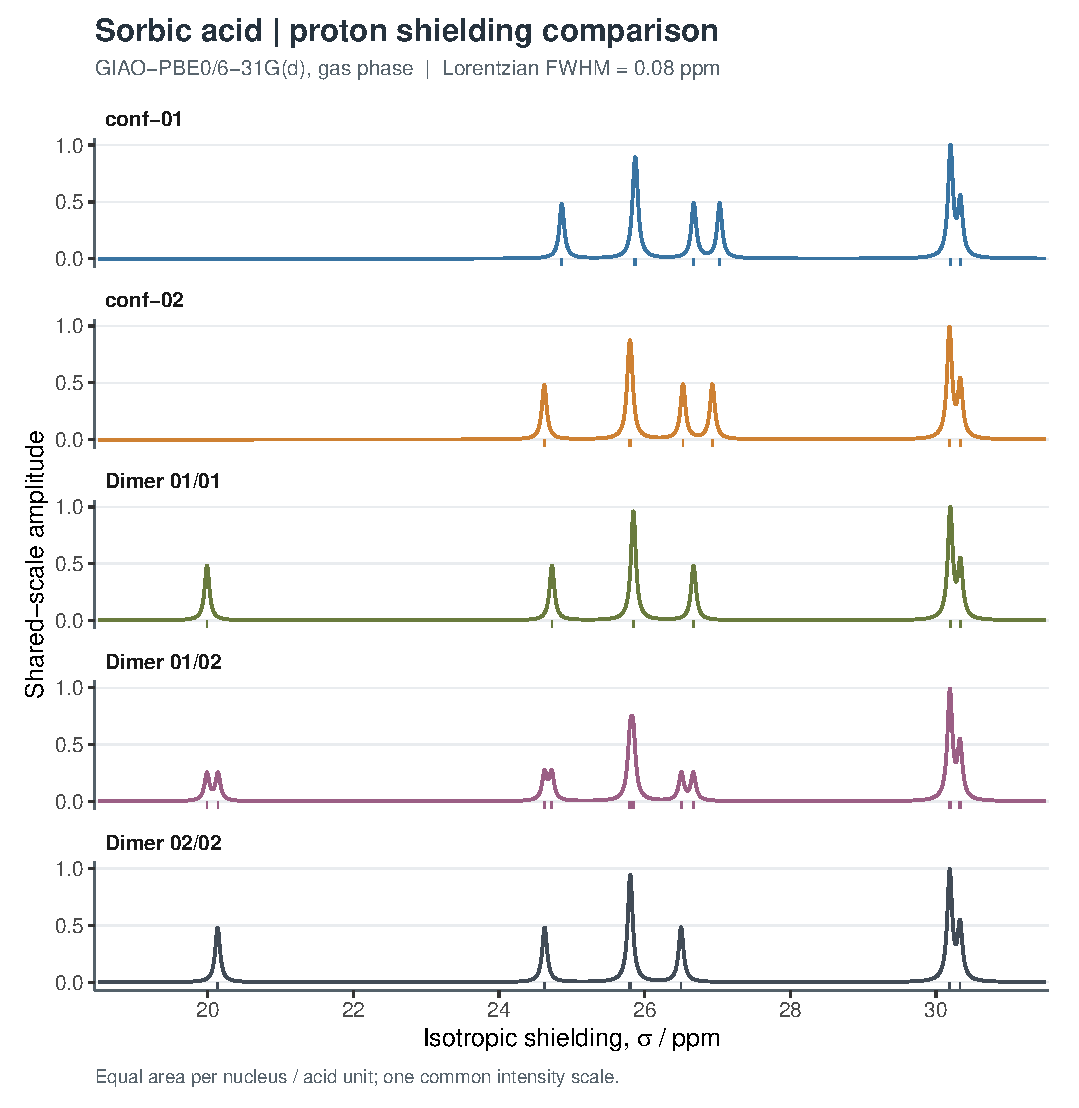
\includegraphics[width=\linewidth]{../analysis/comparison/nmr-H-comparison.pdf}
\caption{单体与二聚体的 $^1$H 屏蔽谱比较。每个核采用等面积线型，二聚体总强度除以 2，再对五条曲线使用同一显示尺度。各行的横轴与纵轴范围一致。}
\label{fig:nhcompare}
\end{figure}
\begin{table}[H]
\centering\small
\caption{羟基氢与羧基碳的屏蔽值（ppm）。01/02 的两项数值分别对应 conf-01 型和 conf-02 型片段；同型二聚体的对应核数值相同。}
\begin{tabular}{lrr}
\toprule
体系 & 羟基氢 $\sigma$ & 羧基碳 $\sigma$\\
\midrule
conf-01 & 27.0304 & 38.8176\\
conf-02 & 26.9311 & 37.4764\\
01/01 & 19.9901 & 31.0808\\
01/02 & 19.9890 / 20.1402 & 31.1973 / 30.3710\\
02/02 & 20.1358 & 30.4664\\
\bottomrule
\end{tabular}
\end{table}
二聚体羟基氢的屏蔽降至约 $20\ \mathrm{ppm}$，相较相应单体降低约 $6.8$--$7.0\ \mathrm{ppm}$，表现为显著的去屏蔽和低场移动。甲基氢的变化很小，羟基位置的变化则远大于 conf-01 与 conf-02 之间的差异。

\clearpage
\begin{figure}[H]
\centering
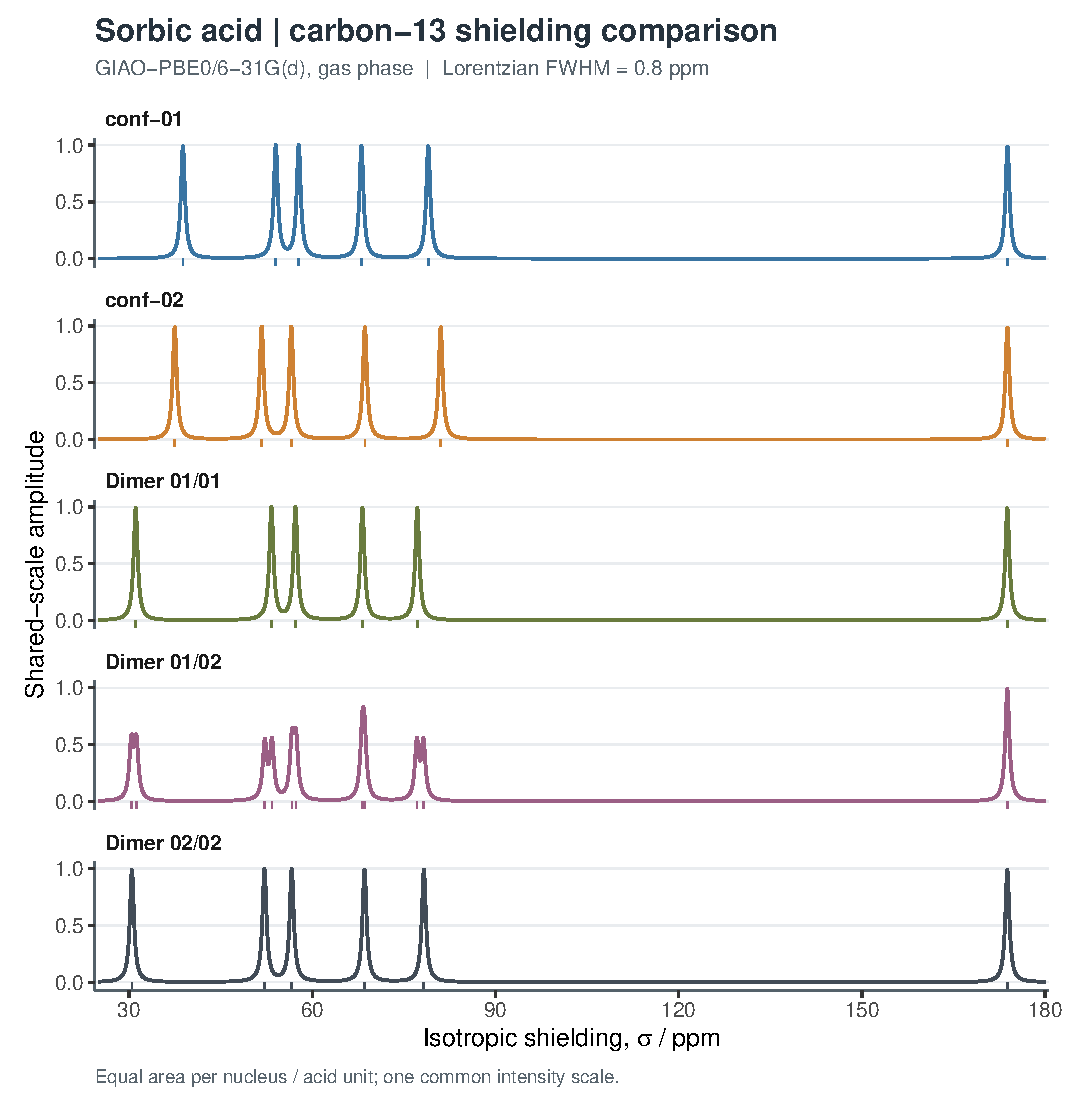
\includegraphics[width=\linewidth]{../analysis/comparison/nmr-C-comparison.pdf}
\caption{单体与二聚体的 $^{13}$C 屏蔽谱比较，强度处理同图\ref{fig:nhcompare}。}
\label{fig:nccompare}
\end{figure}
羧基碳的屏蔽由单体的 $37.48$--$38.82\ \mathrm{ppm}$ 降至二聚体的 $30.37$--$31.20\ \mathrm{ppm}$。01/02 中两个片段的环境不同，若干对应碳核及氢核出现分离；01/01 和 02/02 的对应片段则具有近乎相同的屏蔽值。两种单体及三个二聚体的跨双键烯氢耦合均在 $15.35$--$16.13\ \mathrm{Hz}$ 范围内，双氢键形成并未改变 E/E 构型。

\clearpage
\subsection{与实验氢谱的比较}
实验参考采用国立医药品食品卫生研究所公开研究报告中的山梨酸氢谱\cite{mhlwnmr}：溶剂为 DMSO-$d_6$，测量频率为 $600\ \mathrm{MHz}$，温度为 $25\,^{\circ}\mathrm{C}$，以 DSS-$d_6$ 为内标。原图逐位标注的化学位移列于表\ref{tab:hexp}，原子编号沿用本文从甲基端开始的顺序。
\begin{table}[H]
\centering\small
\caption{实验氢谱的指认及相对甲基的位移差（ppm）。实验值直接取自参考文献的结构标注。}
\label{tab:hexp}
\begin{tabular}{lrrr}
\toprule
位置 & 氢数 & 实验 $\delta$ & $\Delta\delta=\delta-\delta_{\mathrm{CH_3}}$\\
\midrule
H9--H11（甲基） & 3 & 1.84 & 0.00\\
H12 & 1 & 6.26 & 4.42\\
H13 & 1 & 6.26 & 4.42\\
H14 & 1 & 7.18 & 5.34\\
H15 & 1 & 5.79 & 3.95\\
H16（羟基） & 1 & 12.2 & 10.36\\
\bottomrule
\end{tabular}
\end{table}
按式\eqref{eq:relative-shift}得到的实验与理论峰位见图\ref{fig:hexp}。
\begin{figure}[H]
\centering
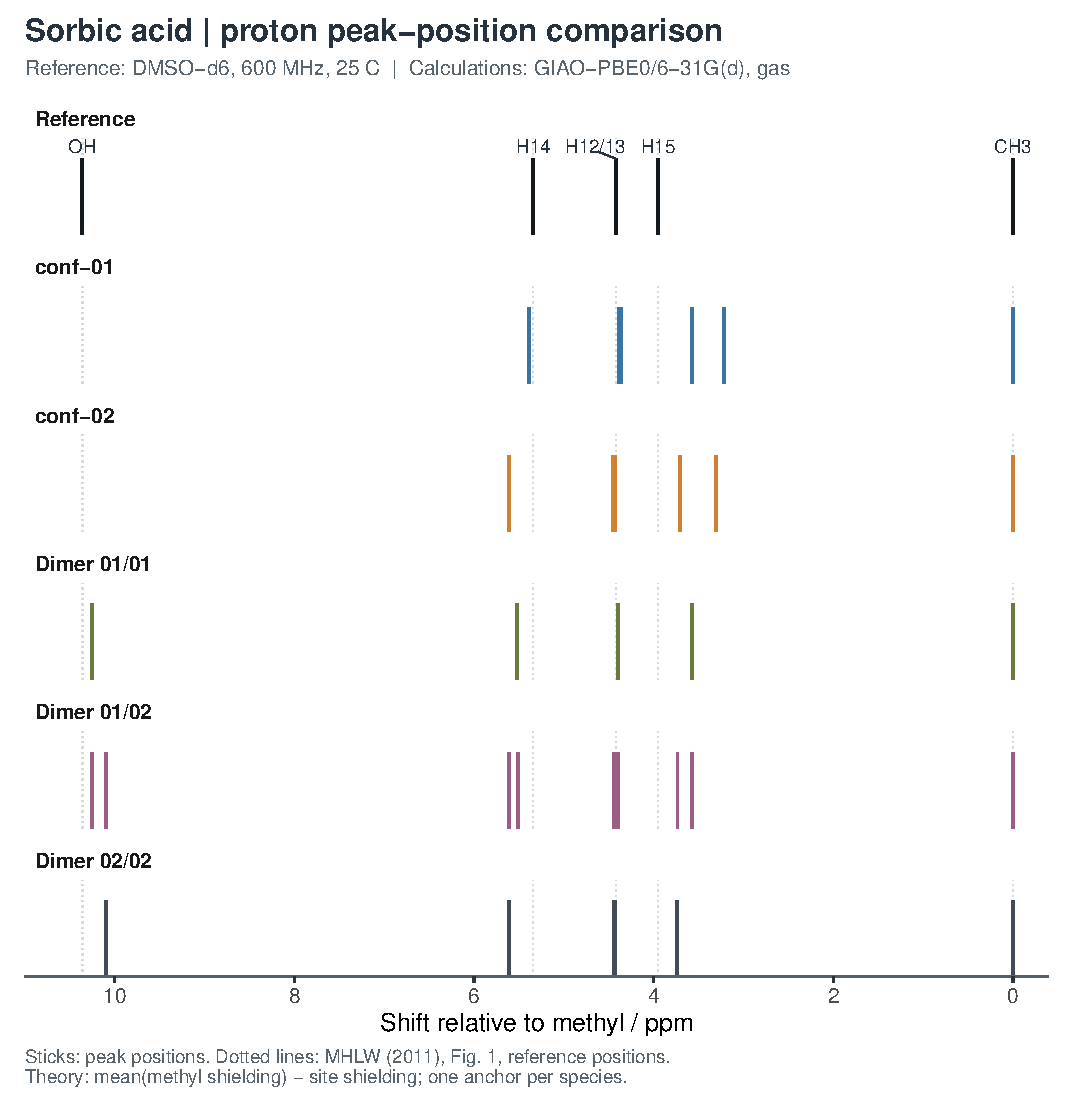
\includegraphics[width=0.96\linewidth]{../analysis/experimental/nmr-H-experiment-comparison.pdf}
\caption{相对甲基的 $^1$H 位移差。等高短棒表示峰位置，虚线标出 DMSO-$d_6$ 溶液中的实验参考值。}
\label{fig:hexp}
\end{figure}

\begin{table}[H]
\centering\small
\caption{相对位移差与实验的比较。烯氢 MAE 为四个烯氢位置的平均绝对偏差，二聚体计入两个片段；不计甲基起点和羟基氢。羟基实验 $\Delta\delta$ 为 10.36 ppm。}
\begin{tabular}{lrr}
\toprule
体系 & 烯氢 MAE / ppm & 羟基 $\Delta\delta^{\mathrm{calc}}$ / ppm\\
\midrule
conf-01 & 0.128 & 3.216\\
conf-02 & 0.138 & 3.306\\
01/01 & 0.150 & 10.254\\
01/02 & 0.141 & 10.250 / 10.099\\
02/02 & 0.128 & 10.102\\
\bottomrule
\end{tabular}
\end{table}
各模型均再现 H14 比其余烯氢更偏低场、H12 与 H13 接近的趋势，烯氢相对位移的平均绝对偏差约为 $0.13$--$0.15\ \mathrm{ppm}$，对这些构象的区分度较低。孤立单体的羟基相对位移仅为 $3.2$--$3.3\ \mathrm{ppm}$，明显小于实验；环状二聚体增大至 $10.1$--$10.3\ \mathrm{ppm}$，表明氢键环境是羟基大幅去屏蔽的重要因素。

DMSO 本身也是氢键受体，实验羟基信号还包含溶质--溶剂氢键和质子交换的影响。因此，这里的二聚体比较主要说明氢键作用的方向和量级。

\subsection{与实验碳谱的比较}
碳谱参考采用 Nishiyama 等报道的 $(2E,4E)$-山梨酸数据\cite{nishiyama}。实验溶剂为 $\mathrm{CDCl_3}$，以 TMS 为内标。原文表 II 的 SOA 栏从羧基端编号，与本文编号顺序相反；对应关系及 conf-02 的逐碳比较列于表\ref{tab:cassignment}。
\begin{table}[H]
\centering\small
\caption{实验碳谱指认与 conf-02 相对位移（ppm）。实验指认沿用原文表 II。}
\label{tab:cassignment}
\begin{tabular}{ccrrr}
\toprule
本文原子 & 文献碳编号 & 实验 $\delta$ & 实验 $\Delta\delta$ & 计算 $\Delta\delta$\\
\midrule
C1 & 6 & 18.70 & 0.00 & 0.00\\
C2 & 5 & 129.73 & 111.03 & 117.26\\
C3 & 4 & 140.74 & 122.04 & 105.21\\
C4 & 3 & 147.34 & 128.64 & 122.12\\
C5 & 2 & 118.25 & 99.55 & 92.80\\
C6 & 1 & 173.00 & 154.30 & 136.36\\
\bottomrule
\end{tabular}
\end{table}
碳谱同样以甲基为参照。采用两种互补的指标：逐碳 MAE 沿用文献原子指认，峰列 MAE 将每个片段的四个烯碳按位移升序配对。前者检验位置归属及位移，后者描述谱峰间距。两者均只计入四个烯碳，结果见表\ref{tab:cexp}。
\begin{figure}[H]
\centering
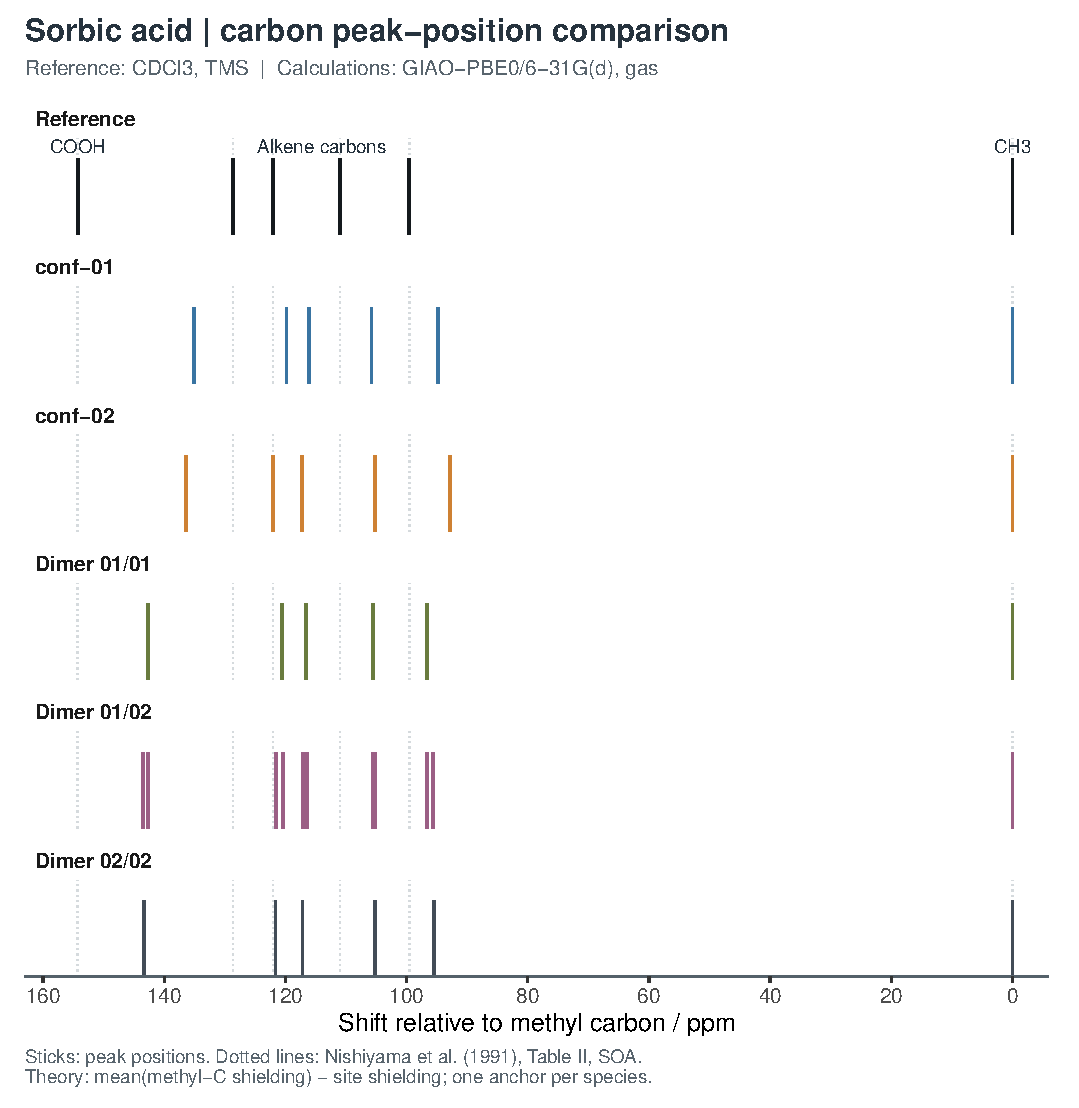
\includegraphics[width=0.96\linewidth]{../analysis/experimental/nmr-C-experiment-comparison.pdf}
\caption{相对甲基碳的 $^{13}$C 位移差。等高短棒表示峰位置，虚线为 $\mathrm{CDCl_3}$ 中的实验参考值。}
\label{fig:cexp}
\end{figure}
\begin{table}[H]
\centering\small
\caption{碳谱相对位移差的比较（ppm）。羧基碳的实验 $\Delta\delta$ 为 154.30；MAE 仅统计烯碳。}
\label{tab:cexp}
\begin{tabular}{lrrr}
\toprule
体系 & 逐碳 MAE & 峰列 MAE & 羧基碳 $\Delta\delta^{\mathrm{calc}}$\\
\midrule
conf-01 & 8.70 & 6.18 & 135.03\\
conf-02 & 9.08 & 5.96 & 136.36\\
01/01 & 8.26 & 5.49 & 142.74\\
01/02 & 8.35 & 5.45 & 142.62 / 143.45\\
02/02 & 8.48 & 5.40 & 143.35\\
\bottomrule
\end{tabular}
\end{table}
所有模型均再现甲基碳、烯碳和羧基碳从高场到低场的分区。单体羧基碳相对甲基的位移差比实验小 $17.94$--$19.27\ \mathrm{ppm}$；加入双氢键后，偏差缩小至 $10.85$--$11.68\ \mathrm{ppm}$，说明缔合增强了羧基碳的去屏蔽。

按文献原指认，烯碳逐碳 MAE 为 $8.26$--$9.08\ \mathrm{ppm}$，高于按峰列配对的 $5.40$--$6.18\ \mathrm{ppm}$。其中 C2 与 C3 的位移次序在所有计算模型中均与文献相反；以 conf-02 为例，两者的相对位移偏差分别为 $+6.23$ 和 $-16.83\ \mathrm{ppm}$。这一差别说明，谱区分布接近与逐碳指认吻合是不同层次的判断。羧基和烯碳的剩余偏差也表明，在当前基组和气相 NMR 模型下，碳谱的定量描述弱于氢谱。

\clearpage
\section{思考与讨论}
\subsection{为什么常用垂直吸收和垂直发射能估计电子光谱？}
电子运动的时间尺度远短于原子核运动。在吸收光子的瞬间，分子核构型来不及显著改变，因此可在基态平衡结构 $R_0$ 上评价两个电子态的能量差。类似地，若发射发生在已弛豫的激发态平衡结构 $R_1$ 附近，垂直发射能可写为 $E_1(R_1)-E_0(R_1)$。这种近似对应 Franck--Condon 图像中的固定核构型电子跃迁，计算成本也低于完整振电光谱。

实际光谱还包含振动精细结构，因此垂直跃迁能一般不等于 0--0 跃迁能。绝热能差比较两个电子态各自平衡结构的能量，进一步计入零点振动能差后才可估计 0--0 能量。

\subsection{理论紫外可见谱与实验谱的差异来自哪些因素？}
泛函和基组影响激发能与振子强度，溶剂及分子几何则改变电子态的相对稳定性。本实验采用气相优化结构上的 SMD 乙醚单点计算；进一步描述溶液光谱，需要考虑溶剂中的几何弛豫、显式氢键和振电耦合。参考带宽约为理论单体带宽的两倍，正体现了统一高斯展宽对真实包络的简化。

单体构象变化使主带移动约 $1.2\ \mathrm{nm}$，双氢键缔合则使其红移约 $8\ \mathrm{nm}$。溶液中各物种的贡献由溶剂、浓度、温度及缔合平衡共同决定。本报告的 UV、氢谱和碳谱来自不同实验条件，因此分别比较各结构的光谱特征，不据此拟合统一的物种比例。

\subsection{理论核磁共振谱与实验谱的差异来自哪些因素？}
相对甲基的位移差消除了参照零点，剩余偏差反映各位置屏蔽响应的差异。氢谱烯氢间距较接近实验，而碳谱的羧基位移及部分烯碳次序存在较大偏差，提示需要进一步检验基组、溶剂环境和文献位点指认。自旋耦合尤其依赖近核电子密度，采用 \texttt{Mixed} 方法所得的两个可比较烯氢耦合与实验相差约 0.4 和 $1.6\ \mathrm{Hz}$。

溶液中的构象交换、甲基转动和振动会产生动态平均，氢键及质子交换则显著影响羟基氢。实验多重峰还与核间耦合、磁等价性、磁场强度及二阶效应有关，峰高和线宽受到弛豫及采集条件的影响。因此，单一气相结构的屏蔽谱与实测 NMR 谱在峰位和线形上均可能存在差异。

\clearpage
\section{实验结论}
在 PBE0/6-31G(d) 水平下，三个山梨酸构象均保持 $(2E,4E)$ 构型并对应局部极小点。conf-02 的电子能最低，conf-01 和 conf-03 分别高出 3.47 和 $26.52\ \mathrm{kJ\,mol^{-1}}$。三个环状二聚体也均无虚频，其中 02/02 的电子能最低。

conf-02 在 SMD 乙醚环境中的主吸收为 $257.44\ \mathrm{nm}$ 的 $S_0\rightarrow S_2$ 跃迁，$f=0.9375$，主要归属为共轭骨架的 $\pi\rightarrow\pi^*$ 激发。两种单体均接近约 $256\ \mathrm{nm}$ 的实验参考峰，二聚体则红移至 $263.53$--$265.31\ \mathrm{nm}$。所选理论展宽明显窄于实验带，带形描述有待进一步考虑振动与溶液环境的贡献。

各模型的烯氢相对位移 MAE 为 $0.13$--$0.15\ \mathrm{ppm}$。conf-02 的两个反式烯氢耦合约为 $15$--$16\ \mathrm{Hz}$；其中 H14--H15 与实验仅相差 $0.42\ \mathrm{Hz}$，支持 E/E 构型。氢键使羟基氢显著去屏蔽，其影响远大于两种低能单体构象之间的差异。

碳谱再现了甲基、烯碳和羧基的分区。二聚体使羧基碳相对位移更接近实验，但仍低估约 $11\ \mathrm{ppm}$；按文献指认，烯碳逐碳 MAE 为 $8.26$--$9.08\ \mathrm{ppm}$，且 C2、C3 的次序与计算相反。总体上，当前模型较好描述了主 UV 峰位、烯氢间距和主要耦合，对氢键效应给出了明确趋势，而碳谱的逐位定量一致性较弱。

\begin{thebibliography}{9}
\small
\bibitem{course} 刘迎春. 山梨酸紫外光谱与核磁共振谱的计算. 浙江大学量子化学实验课程讲义, 2026, 第7--16页.
\bibitem{nmr} Gaussian, Inc. NMR keyword: GIAO, SpinSpin and Mixed options. Gaussian 用户手册（镜像）. \url{https://tungsten.ch.uj.edu.pl/doc/g09doc/g09ur/k_nmr.htm}.
\bibitem{deng} Deng W, Cheeseman J R, Frisch M J. Calculation of Nuclear Spin-Spin Coupling Constants of Molecules with First and Second Row Atoms in Study of Basis Set Dependence. \textit{J. Chem. Theory Comput.}, 2006, 2(4): 1028--1037. \url{https://doi.org/10.1021/ct600110u}.
\bibitem{nistuv} Timmons C J. \textit{UV Atlas of Organic Compounds}, 1966, 1: B7/1. 山梨酸 UV 数据收录于 NIST Chemistry WebBook, SRD 69, RAS UV No. 19947. \url{https://webbook.nist.gov/cgi/cbook.cgi?ID=C110441&Mask=400}. 访问日期：2026-10-09.
\bibitem{mhlwnmr} 大槻崇. NMRを用いた食品中の食品添加物分析法の開発に関する研究. 平成22年度総括研究報告書. 国立医薬品食品衛生研究所, 2011年4月, 图1（第11页）、表1（第16页）. \url{https://mhlw-grants.niph.go.jp/system/files/2010/104031/201033054A/201033054A0001.pdf}.
\bibitem{nishiyama} Nishiyama Y, Tamura Y, Ibe A, et al. Study on Isomers of Sorbic Acid Produced in Food. \textit{Eisei Kagaku}, 1991, 37(2): 89--96, 表 II、III（第93页）. \url{https://doi.org/10.1248/jhs1956.37.89}.
\end{thebibliography}

\clearpage
\appendix
\section{conf-02 的激发态数据}
\begin{table}[H]
\centering\small
\caption{conf-02 在 SMD 乙醚环境中最低 20 个激发单重态。}
\begin{tabular}{rrrr}
\toprule
激发态 & 激发能 / eV & 波长 / nm & 振子强度 $f$\\
\midrule
1 & 4.7257 & 262.36 & 0.0001\\
2 & 4.8160 & 257.44 & 0.9375\\
3 & 6.4992 & 190.77 & 0.0122\\
4 & 6.8562 & 180.83 & 0.0000\\
5 & 6.9150 & 179.30 & 0.0888\\
6 & 7.4409 & 166.62 & 0.0011\\
7 & 7.5534 & 164.14 & 0.0676\\
8 & 7.6346 & 162.40 & 0.0001\\
9 & 7.7194 & 160.61 & 0.0007\\
10 & 8.2595 & 150.11 & 0.0021\\
11 & 8.4402 & 146.90 & 0.0001\\
12 & 8.7735 & 141.32 & 0.0006\\
13 & 8.9086 & 139.17 & 0.0150\\
14 & 9.1008 & 136.23 & 0.0079\\
15 & 9.1037 & 136.19 & 0.0319\\
16 & 9.2173 & 134.51 & 0.0015\\
17 & 9.3107 & 133.16 & 0.0138\\
18 & 9.3952 & 131.96 & 0.0000\\
19 & 9.5610 & 129.68 & 0.0278\\
20 & 9.5931 & 129.24 & 0.0005\\
\bottomrule
\end{tabular}
\end{table}
表中振子强度保留四位小数，$0.0000$ 表示该跃迁在此精度下极弱。
\end{document}
